% Drivers.tex
The workhorses of the \Gfour{} visualization system continues to be its OpenGL
drivers.  Multiple OpenGL drivers are provided because different implementations
are required on different operating systems or for different user memory 
configurations.  For example, one flavor of OpenGL driver offers higher refresh
speed at the cost of using more memory, while another conserves memory at the
cost of speed.  The user experience has been simplified so that it is no longer 
necessary to specify which driver to use (such as /vis/open OGLI or 
/vis/open OGLSWin32).  Instead a single command (/vis/openOGL) may be issued 
from which \Gfour{} will select the most appropriate and capable viewer for the
user's current system.

Other improvements include speed increases through the streamlining of the set
of OpenGL instructions, and the ability to print any OpenGL view to high quality
output by exploiting the GL2PS \cite{vis:GL2PS} OpenGL to PostScript printing 
library.  OpenGL drivers in X11 and Qt modes allow the user to select (``pick'')
objects from the GUI in order to interrogate visualized objects, thus obtaining
track, hit or geometry information.

\Gfour{} now supports wrapping an OpenGL viewer within the versatile, highly
interactive and platform-independent Qt user interface framework.  An example of
this is shown in Figure \ref{fig:vis1}.

\begin{figure}
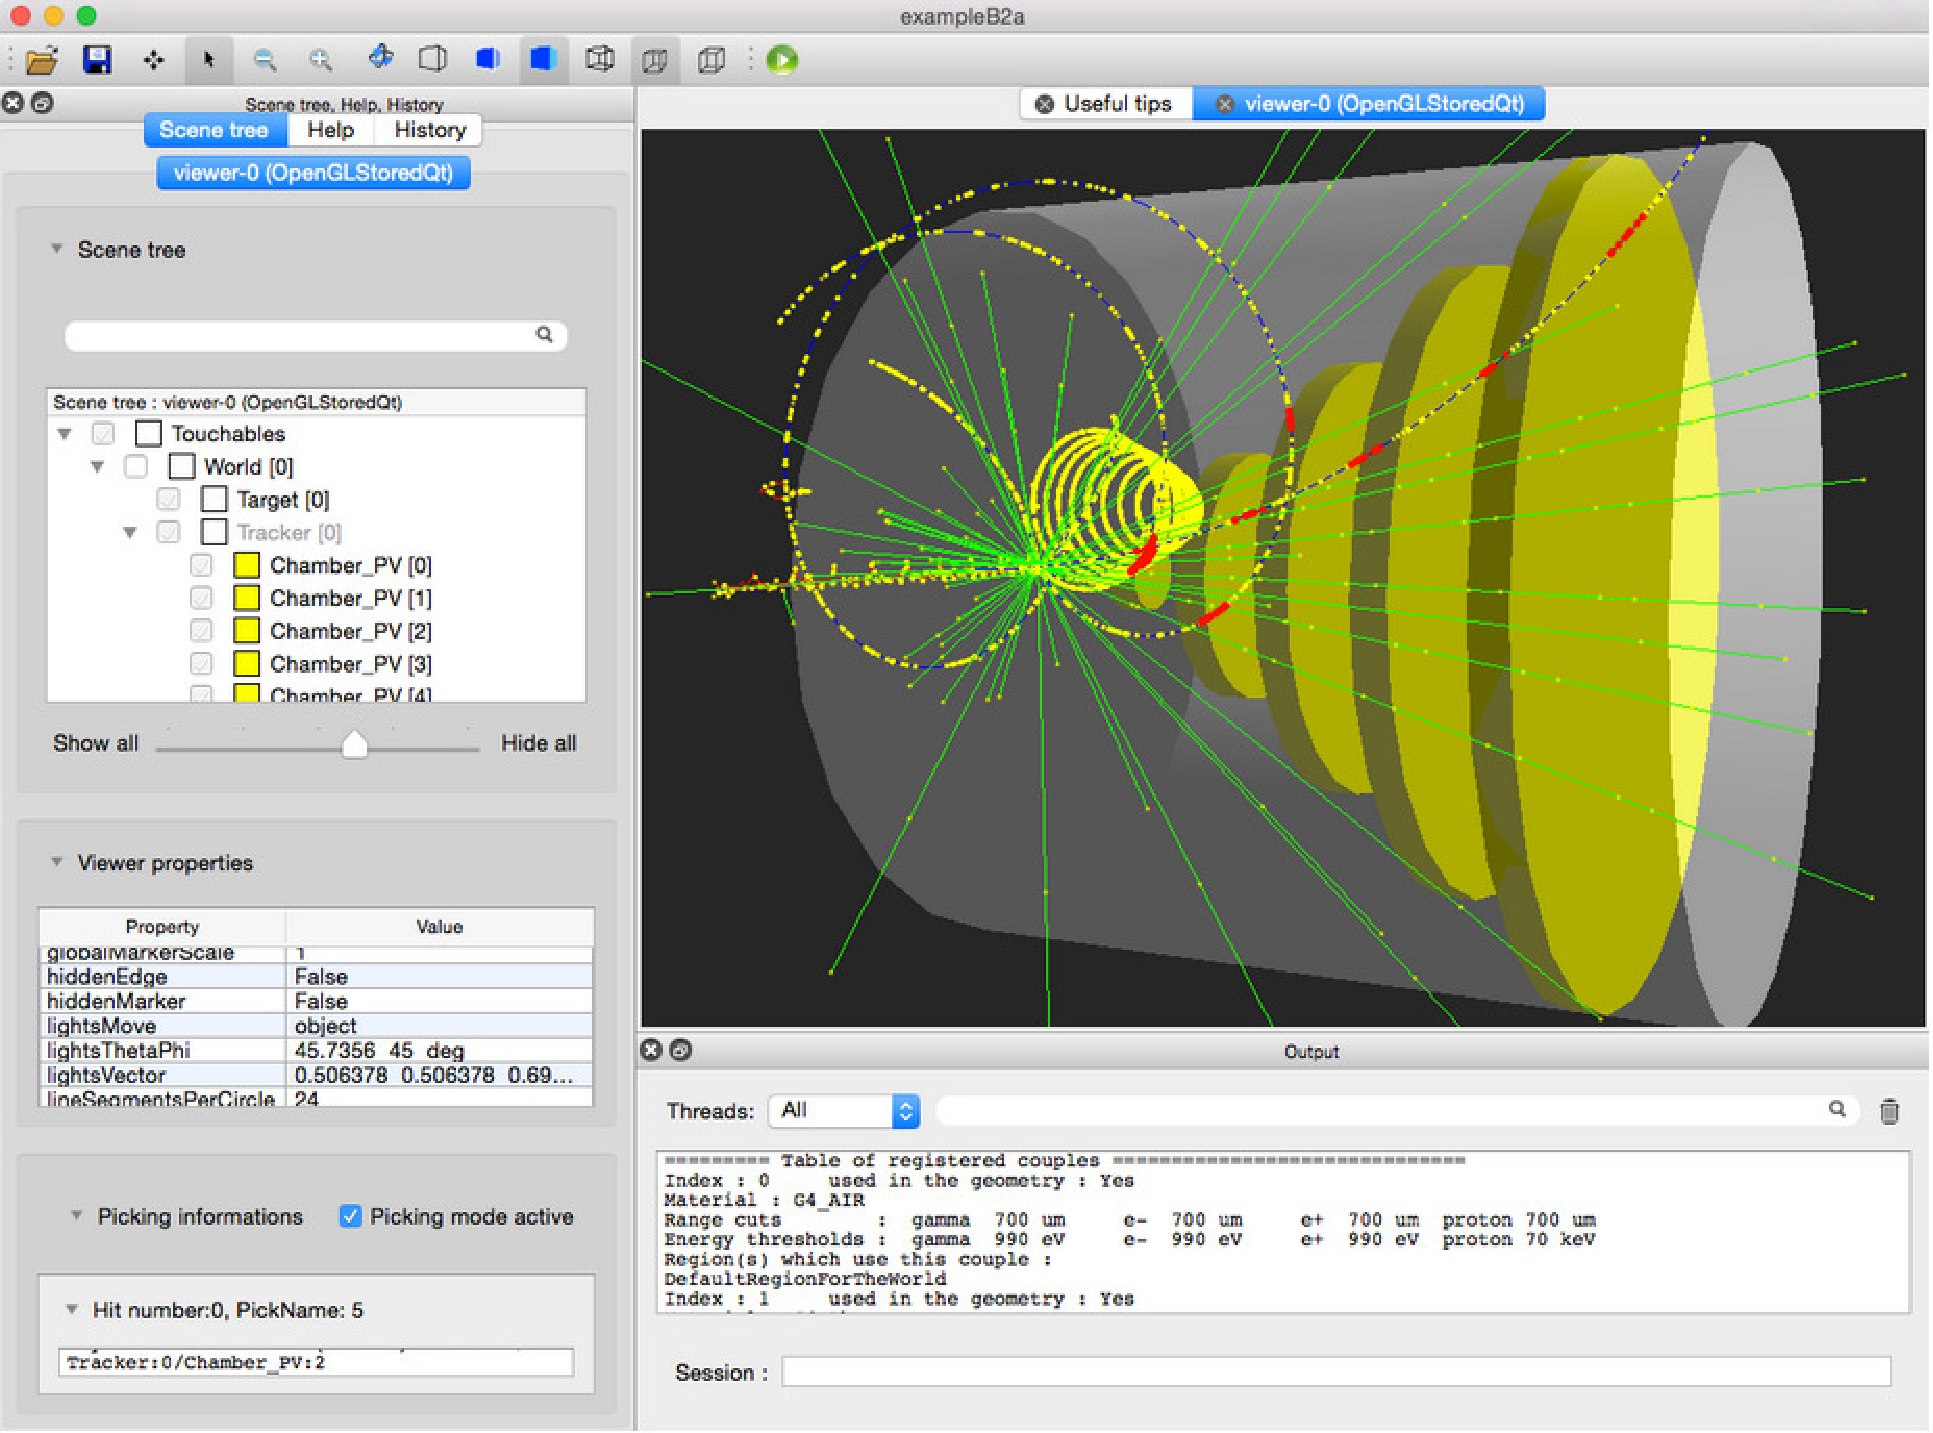
\includegraphics[width=0.47\textwidth]{figures/visfig1.pdf}
  \caption{Screenshot of OpenGL viewer wrapped in Qt.}
  \label{fig:vis1}
\end{figure}
This Qt implementation includes GUI functionality to rotate, zoom and translate
the view, and to pick visualization objects.  A slider lets the user visually
``melt away'' layers of hierarchical geometries.  Movies and EPS output are 
easily generated.  A hierarchical view of the scene's graphical elements allows 
the user to inspect and modify the color and visibility of each element.  
Another hierarchical view provides easy access to the full \Gfour{} help system.

\begin{figure}
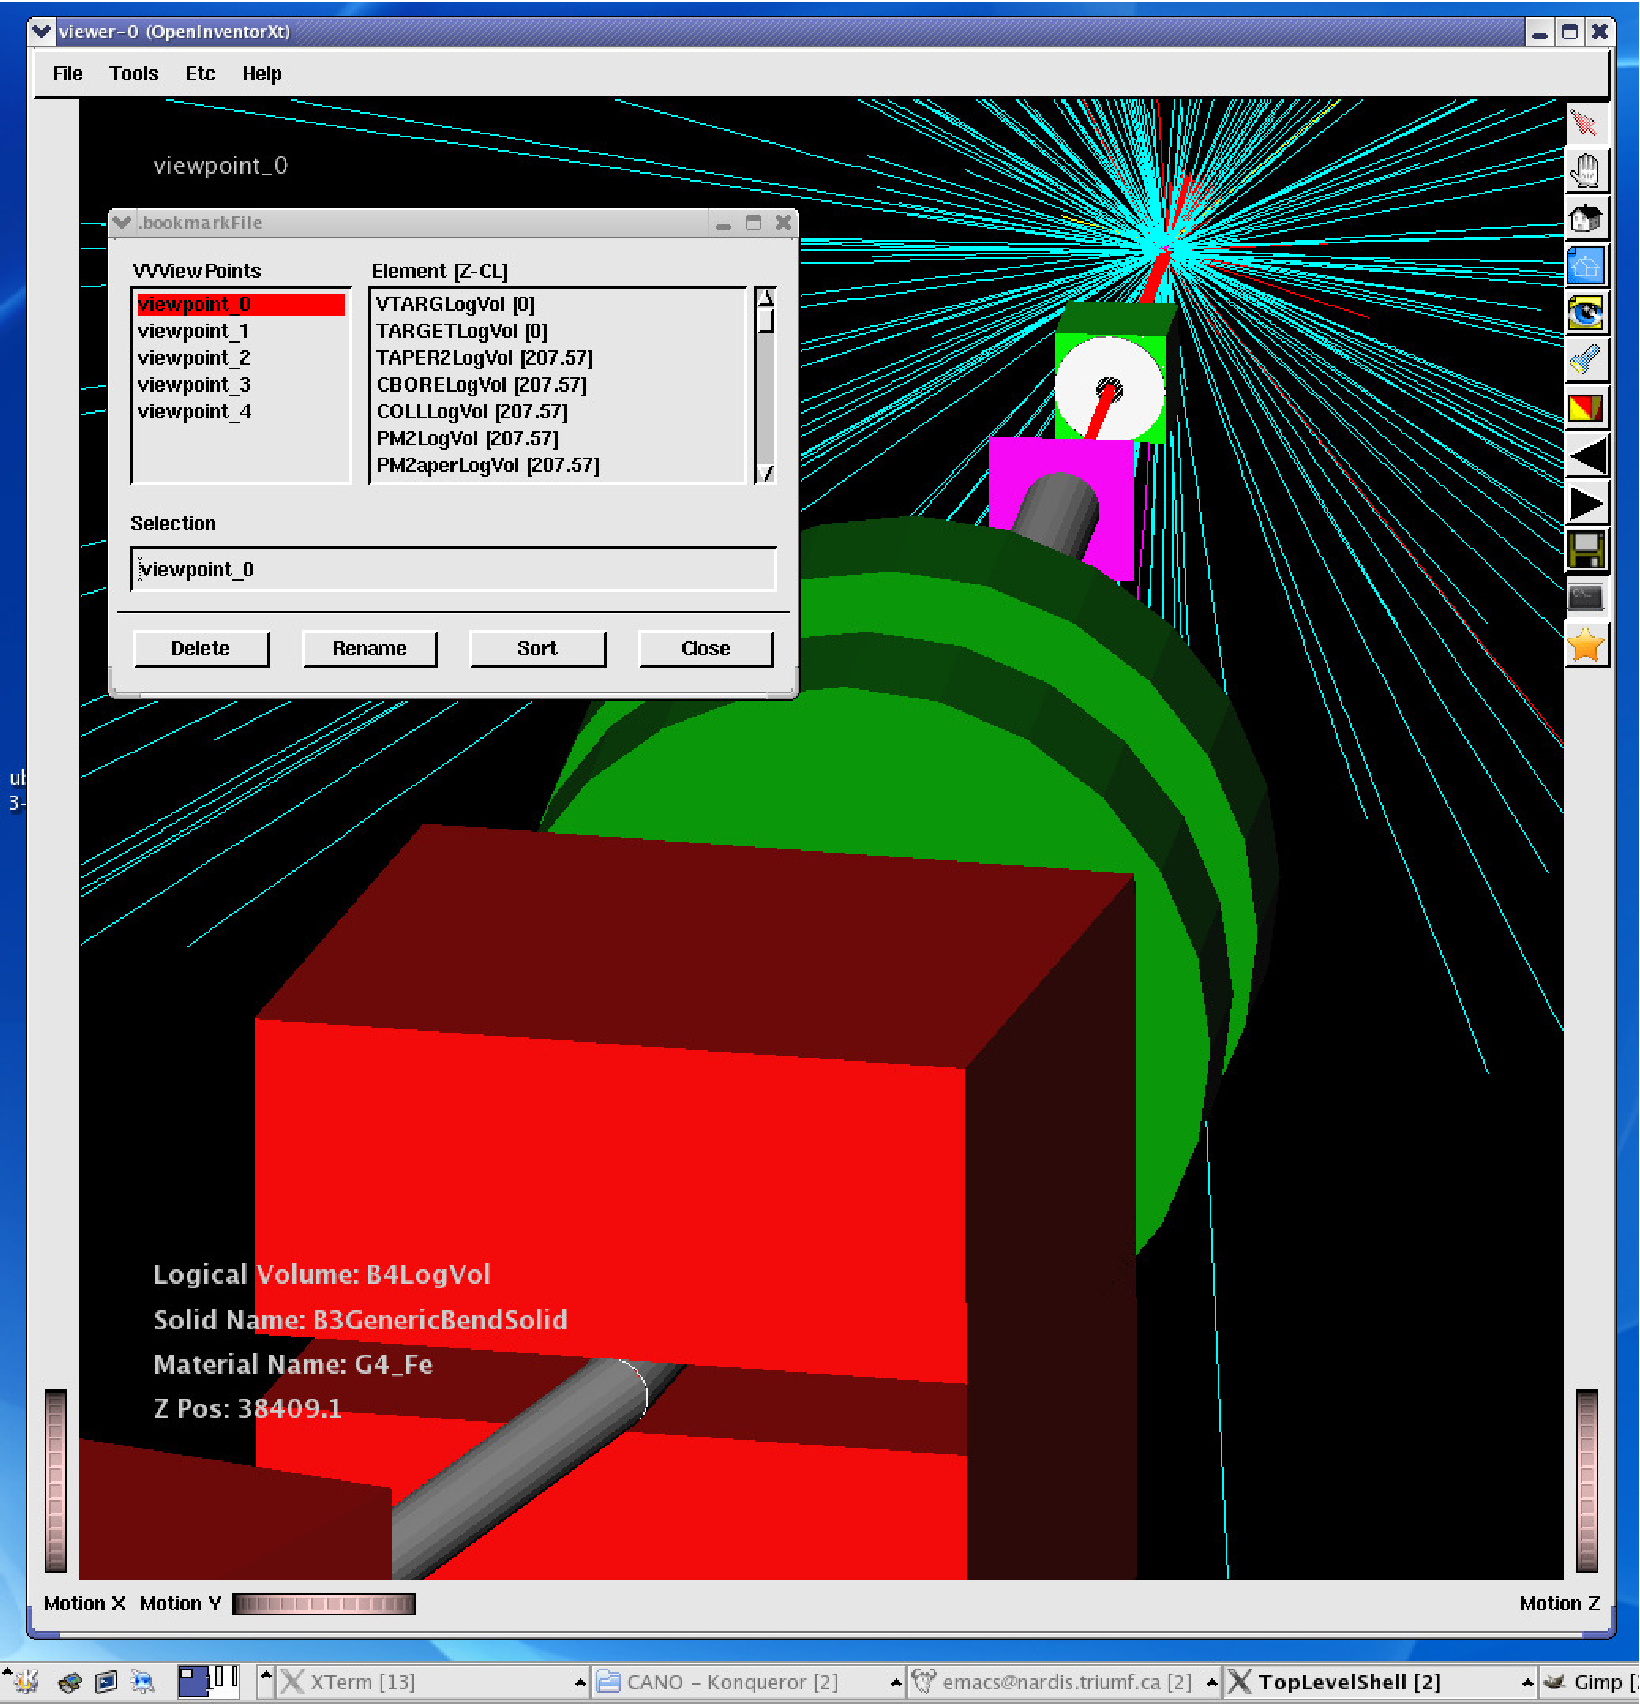
\includegraphics[width=0.47\textwidth]{figures/visfig2.pdf}
  \caption{Screenshot of Open Inventor Extended viewer.}
  \label{fig:vis2}
\end{figure}

New features have also been added to the Open Inventor (OI) driver.  The 
availability of OI greatly improved in 2011 when the Coin3D \cite{vis:coin3d} 
version of these libraries became open-source and freely available.  \Gfour{} 
made extensive use of the Coin3D classes that extend the original SGI OI 
library, creating a distinct new ``extended'' driver OIXE while leaving the 
basic driver OIX unchanged.  Figure \ref{fig:vis2} shows an example of the OIXE
viewer. 

A feature implemented in this area was the ability to save the current view and
return to it at any later time in the current or future runs.  Views are saved 
and accumulated in a bookmarks file specified by the user.  Each view is tagged
with a user-provided or default name, and all views are listed in a scrolling 
auxiliary window.  Clicking on a view name restores the view, or a sequence of 
views can be walked through via the keyboard's arrow keys.  All viewpoint and 
camera parameters are stored in ASCII form allowing editing or external 
generation of bookmarks.

As in other OpenGL viewers, object selection from the GUI is supported on 
trajectories, hits and geometry.  The OI driver provides both normal trajectory 
picking, where all trajectory points are shown, and reduced picking, where only
the first and last points are shown.  The viewer also supports mouse-over 
picking, whereby the element data is displayed directly in the viewer window 
when the mouse pointer is hovered over any object.

The remaining new developments concern moving the camera along a reference
path.  They are motivated by accelerator and beam line geometries, but may be
useful for other large and/or extended structures.  The reference path, defined
in a piecewise linear fashion by an ordered set of points, may be read from a 
file or copied from any particle trajectory.  Once a reference path is 
established, a navigation panel lists all elements in the geometry, ordered by
their distance along the reference path (based on the shortest distance 
\cite{vis:polyline} from the element center to the path).  The panel may then
be used to extract information on the elements or rotate the camera around them.
% moves the camera immediately to a centered view of that 
% element, and the arrow keys can then be used to rotate the camera around the 
% element in precise 90-degree steps around the local axes.  The shifted left and
% right arrow keys provide smooth movement of the camera along the reference path.
% OI capabilities have been used to render these motions smoothly so as not to be
% jarring to the eye.  During camera movement, a continuous readout of the 
% distance along the reference path is given.

A Reference Path Animation mode moves the camera continuously along the path, 
allowing a fly-through giving a particle's-eye view of the geometry.  Keyboard 
controls adjust animation speed and direction and allow adjusting the camera 
angle to obtain fly-overs and fly-unders.

